\begin{figure}[h!]
    \centering
    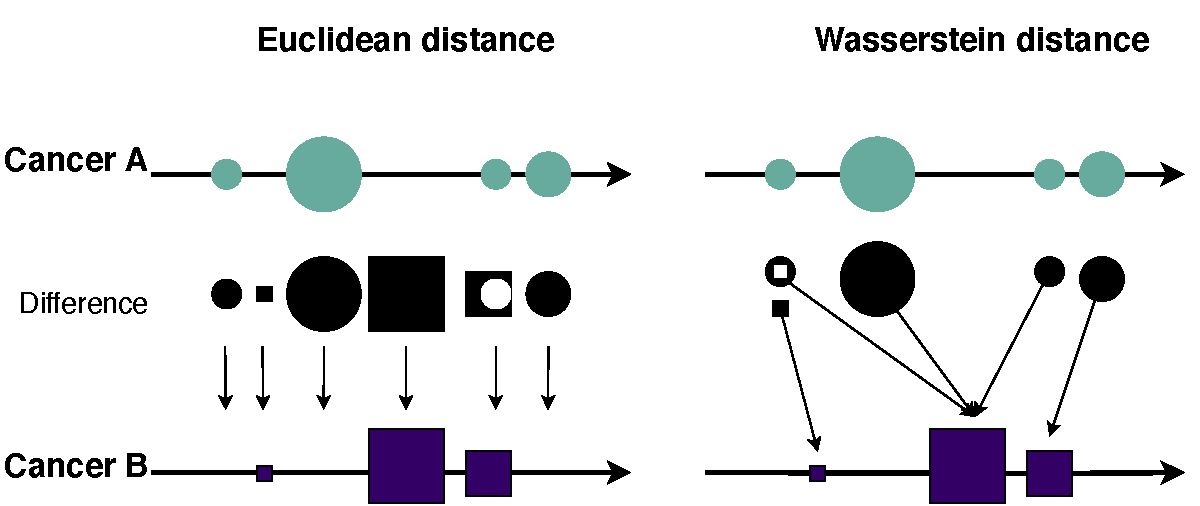
\includegraphics[scale=0.7]{graphics/wasserstein_demo.pdf}
    \caption{\textbf{Schematic diagram for Euclidean and Wasserstein distance between two vectors.} Euclidean is the point-wise difference between the same location on vectors A and B, and is strictly in the vertical direction. Wasserstein is takes into account both the vertical and horizontal directions; it is intuitively the minimal amount of work required to transport mass from A to B.}
    \label{fig:wasserstein_demo}
\end{figure}
